\documentclass[12pt,letterpaper]{exam}
\usepackage[lmargin=1in,rmargin=1in,tmargin=1in,bmargin=1in]{geometry}
\usepackage{../style/exams}

% -------------------
% Course & Exam Information
% -------------------
\newcommand{\course}{MAT 107: Exam 1}
\newcommand{\term}{Winter -- 2022}
\newcommand{\examdate}{01/08/2023}
\newcommand{\timelimit}{Time Limit: `$\infty$'}

\setbool{hideans}{true} % Student: True; Instructor: False

% -------------------
% Content
% -------------------
\begin{document}

\examtitle
\instructions{Write your name on the appropriate line on the exam cover sheet. This exam contains \numpages\ pages (including this cover page) and \numquestions\ questions. Check that you have every page of the exam. Answer the questions in the spaces provided on the question sheets. Be sure to answer every part of each question and show all your work. If you run out of room for an answer, continue on the back of the page --- being sure to indicate the problem number.} 
\scores
\bottomline
\newpage

% ---------
% Questions
% ---------
\begin{questions}

% Question 1
\newpage
\question[10] Construct the logic table for $P \to (\neg P \vee Q)$. 



% Question 2
\newpage
\question[10] Show that $\neg (P \to Q)$ and $P \wedge \neg Q$ are logically equivalent. 



% Question 3
\newpage
\question[10] Find the logical expression corresponding to the following circuit:



% Question 4
\newpage
\question[10] Find a logical expression corresponding to a circuit whose on/off table is given below: \par
	\begin{table}[h]
	\centering
	\begin{tabular}{c|c|c|c}
	$P$ & $Q$ & $R$ & ? \\ \hline
	$1$ & $1$ & $1$ & $1$ \\
	$1$ & $1$ & $0$ & $0$ \\
	$1$ & $0$ & $1$ & $0$ \\
	$1$ & $0$ & $0$ & $0$ \\
	$0$ & $1$ & $1$ & $0$ \\
	$0$ & $1$ & $0$ & $1$ \\
	$0$ & $0$ & $1$ & $0$ \\
	$0$ & $0$ & $0$ & $1$
	\end{tabular}
	\end{table}



% Question 5
\newpage
\question[10] Convert the following to base-10:
	\begin{enumerate}[(a)]
	\item $1110011_2$
	\item $4501_6$
	\item $\texttt{ca}1_{16}$
	\end{enumerate}



% Question 6
\newpage
\question[10] Convert the following base-10 numbers to the indicated base-$b$ numbers:
	\begin{enumerate}[(a)]
	\item $27$, $b= 2$
	\item $654$, $b= 7$
	\item $1492$, $b= 16$
	\end{enumerate}



% Question 7
\newpage
\question[10] Consider a subtraction game with perfect players and subtraction $S= \{ 1, 3, 5 \}$. Show you go first or second if there are 2023 coins? If you should go first, what is a winning move? 



% Question 8
\newpage
\question[10] Explain why you should go first in the game of NIM below. What is a winning opening move?
	\[
	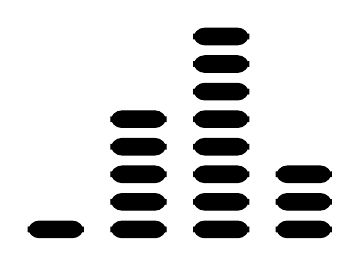
\begin{tikzpicture}[scale=0.7]
	% First Pile
	\draw[rounded corners,fill=black] (0,0) rectangle (1,0.3);
	% Second Pile
	\draw[rounded corners,fill=black] (1.5,0) rectangle (2.5,0.3);
	\draw[rounded corners,fill=black] (1.5,0.5) rectangle (2.5,0.8);
	\draw[rounded corners,fill=black] (1.5,1) rectangle (2.5,1.3);
	\draw[rounded corners,fill=black] (1.5,1.5) rectangle (2.5,1.8);
	\draw[rounded corners,fill=black] (1.5,2) rectangle (2.5,2.3);
	% Third Pile
	\draw[rounded corners,fill=black] (3,0) rectangle (4,0.3);
	\draw[rounded corners,fill=black] (3,0.5) rectangle (4,0.8);
	\draw[rounded corners,fill=black] (3,1) rectangle (4,1.3);	
	\draw[rounded corners,fill=black] (3,1.5) rectangle (4,1.8);	
	\draw[rounded corners,fill=black] (3,2) rectangle (4,2.3);	
	\draw[rounded corners,fill=black] (3,2.5) rectangle (4,2.8);	
	\draw[rounded corners,fill=black] (3,3) rectangle (4,3.3);	
	\draw[rounded corners,fill=black] (3,3.5) rectangle (4,3.8);	
	% Fourth Pile
	\draw[rounded corners,fill=black] (4.5,0) rectangle (5.5,0.3);
	\draw[rounded corners,fill=black] (4.5,0.5) rectangle (5.5,0.8);
	\draw[rounded corners,fill=black] (4.5,1) rectangle (5.5,1.3);	
	\end{tikzpicture}
	\]



% Question 9
\newpage
\question[10] Nancy and Drew are taking out a simple discount note to pay for a cruise. This loan will be for \$3,800 for 3~months at 9.6\% yearly interest. How much do they receive from the bank? 



% Question 10
\newpage
\question[10] Suppose that you invest \$7,000 into an account which earns 2.3\% annual interest, compounded quarterly. Will you have \$10,000 in the account after 6~years? Explain. If not, how long until the account contains \$10,000?


\end{questions}
\end{document}